\documentclass[10pt]{article}
\input{style/coursHeadings}
\input{style/programHeadings}
\input{style/macros_SII}
\input{style/macros_Titres}
\input{style/macros_Frames}

%Si le boolen xp est vrai : compilation pour xabi
%Sinon compilation Damien
\newboolean{xp}
\setboolean{xp}{true}

\newboolean{prof}
\setboolean{prof}{false}

\usepackage[%
    pdftitle={CI 06 : Stat - Modélisation des AM},
    pdfauthor={Xavier Pessoles},
    colorlinks=true,
    linkcolor=blue,
    citecolor=magenta]{hyperref}


\def\discipline{Sciences Industrielles de l'Ingénieur}
\def\xxtitre{\ifthenelse{\boolean{xp}}{
CI 06 : Étude du comportement statique des systèmes}{}}

\def\xxsoustitre{\ifthenelse{\boolean{xp}}{
Chapitre 1 -- Modélisation des Actions Mécaniques}{
Partie  -- }}

\def\xxauteur{\ifthenelse{\boolean{xp}}{
%Xavier \textsc{Pessoles}
}{}}

\def\xxpied{\ifthenelse{\boolean{xp}}{
CI 06 : Statique\\
Ch. 2 : PFS -- Application -- Coussinets}{
\xxtitre}}

\def\xxcathegorie{\ifthenelse{\boolean{xp}}{
2013 -- 2014 \\
Xavier \textsc{Pessoles}}{}}

%---------------------------------------------------------------------------

\begin{document}

\ifthenelse{\boolean{xp}}{\input{style/enteteXP}}{\input{style/enteteDI}}

\begin{center}
\Large{\textsc{Exercices d'applications : Choix de coussinet}}
\end{center}

\vspace{.25cm}

\section*{Choix de coussinets -- Engrenage à denture droite}

\begin{obj}
\begin{itemize}
\item Déterminer le couple moteur nécessaire.
\item Choisir les coussinets.
\end{itemize}
\end{obj}


Le schéma d'architecture du montage ci-dessous présente un pignon arbré entraîné par un moteur (non représenté). La fréquence de rotation de l'arbre est de 180 tr/min.
L'effort à transmettre par l'engrenage est de 2400N. L'angle de pression dans l'engrenage est de 20\textdegree. On a $\vect{AB} = 3a \vect{z}$ et $\vect{AC} = R \vect{y}$.

\begin{center}
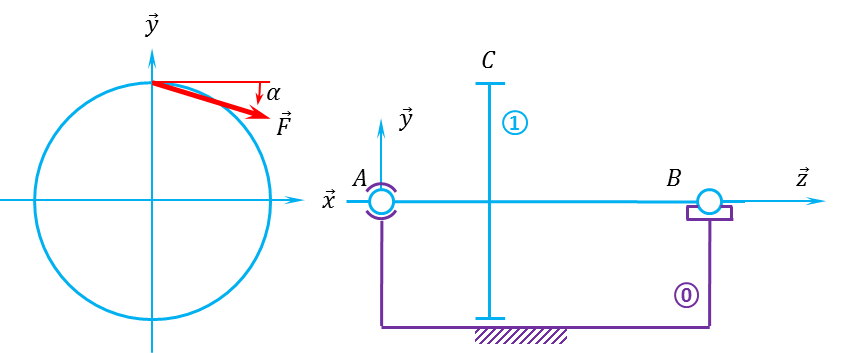
\includegraphics[width=.75\textwidth]{images/modele}
\end{center}

\subsection*{Détermination des actions mécaniques}

\subparagraph{}
\textit{Isoler l'arbre et faire le bilan des actions mécaniques.}

\subparagraph{}
\textit{Appliquer le PFS.}

\subparagraph{}
\textit{Déterminer les actions mécaniques dans les liaisons ainsi que le couple moteur nécessaire ?}

\subparagraph{}
\textit{Aurait-il été possible de trouver les actions mécaniques plus rapidement ?}

\subsection*{Choix des coussinets}
Un calcul en torsion de l'arbre impose un diamètre supérieur à 30 mm. 
Les dimensions du mécanisme imposent $a=50\; mm$.

On désire savoir si un certain type de coussinet pourrait être utilisé :
\begin{itemize}
\item diamètre nominal intérieur du coussinet : 35 mm;
\item diamètre nominal extérieur du coussinet : 39 mm;
\item longueurs de coussinet disponibles : 20, 30, 35 et 50 mm.
\end{itemize}

La pression maximale admissible entre l'arbre et le coussinet est de 14 MPa. Le constructeur impose que le produit pV (pression multipliée par la vitesse) soit inférieur à 0,7 Mpa m/s.

\subparagraph{}
\textit{Est-il possible d'utiliser un des coussinets proposés ?}


\section*{Choix de coussinets -- Engrenage à denture hélioïdale}

\begin{obj}
\begin{itemize}
\item Déterminer le couple moteur nécessaire.
\item Choisir les coussinets.
\end{itemize}
\end{obj}


Le schéma d'architecture du montage ci-dessous présente un pignon conique relié à un arbre,  entraîné par un moteur (non représenté). La fréquence de rotation de l'arbre est de 120 tr/min.

La résultante des efforts au point $A$ est donné par $\vect{F_A} = -10\,000\vect{x} +3200\vect{y} + 1700\vect{z}$.

\begin{center}
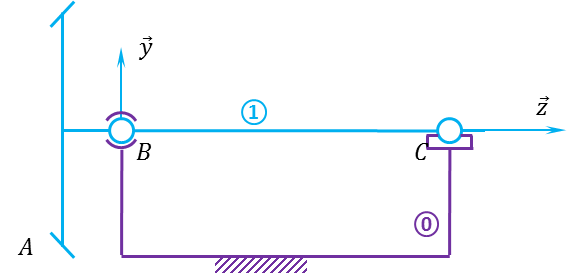
\includegraphics[width=.75\textwidth]{images/modele2}
\end{center}

\subsection*{Détermination des actions mécaniques}

\subparagraph{}
\textit{Déterminer les actions mécaniques dans les paliers en $B$ et $C$.}

\subsection*{Choix des coussinets}
Le concepteur du montage impose que le rapport entre la longueur de guidage et le diamètre du coussinet soit compris entre 0,6 et 0,8.

Un constructeur de coussinets donne les conditions de fonctionnement suivante : 
\begin{itemize}
\item $p_{max}=18 \; MPa$;
\item $V_{maxi}= 6\; m\cdot s^{-1}$;
\item $(pV)_{maxi} = 1,8 MPa \; \cdot m\cdot s^{-1}$.
\end{itemize}

\subparagraph{}
\textit{Déterminer les dimensions d'un coussinet à collerette en $B$ et d'un coussinet sans collerette en $C$.}


\end{document}


